\chapter{TINJAUAN PUSTAKA}

\section{Landasan Teori}

\subsection{Traffic Engineering}
\textit{Traffic Engineering} (TE) adalah disiplin rekayasa jaringan yang berfokus pada pengukuran, pemodelan, karakterisasi, dan kontrol lalu lintas internet untuk mengoptimalkan kinerja jaringan. Tujuan utama TE adalah meminimalkan kongesti dan meningkatkan pemanfaatan sumber daya melalui penyeimbangan beban trafik (\textit{load balancing}) \cite{marouani2024}.

TE modern membutuhkan kemampuan untuk menangani pola trafik yang dinamis dan beragam, di mana pendekatan konvensional berbasis algoritma statis seperti jalur terpendek (Dijkstra) seringkali tidak mampu beradaptasi dengan kondisi jaringan yang berubah secara real-time. Oleh karena itu, pendekatan berbasis kecerdasan buatan semakin diperlukan untuk melakukan optimasi distribusi trafik secara adaptif dan efisien.

\begin{figure}[H]
    \centering
    \includegraphics[width=0.8\textwidth]{images/te.png}
    \caption{Ilustrasi Traffic Engineering dalam Jaringan}
    \label{fig:traffic_engineering}
\end{figure}

\subsection{Jaringan Layer 2 dan VLAN}
Jaringan Layer 2 beroperasi pada lapisan \textit{Data Link} dalam model OSI, di mana perangkat \textit{switch} mengirimkan frame berdasarkan alamat MAC\@. Teknologi VLAN (\textit{Virtual Local Area Network}) memungkinkan segmentasi jaringan secara logis dalam satu infrastruktur fisik, meningkatkan keamanan dan efisiensi manajemen jaringan. Segmentasi VLAN terbukti dapat meningkatkan performa jaringan dengan membagi \textit{broadcast domain} yang besar menjadi domain-domain yang lebih kecil dan terkelola \cite{warse2025vlan}.

Pada lingkungan ISP yang menggunakan infrastruktur \textit{switching} Layer 2 dengan VLAN, penerapan Traffic Engineering menghadapi tantangan khusus. Mekanisme \textit{Spanning Tree Protocol} (STP) pada Layer 2 cenderung memblokir jalur redundan untuk mencegah \textit{looping}, yang mengakibatkan tautan cadangan tidak termanfaatkan (\textit{underutilized}) \cite{rashid2024performance, aruba2025campus}. Meskipun varian yang lebih modern seperti \textit{Rapid Spanning Tree Protocol} (RSTP) menawarkan konvergensi yang lebih cepat, kondisi ini tetap membuat optimasi jalur menjadi lebih kompleks dibandingkan jaringan IP tradisional (Layer 3) \cite{ahmad2020intervlan}. Oleh karena itu, diperlukan pendekatan cerdas untuk memprediksi kegagalan dan mendistribusikan trafik secara dinamis tanpa melanggar topologi logis Layer 2 \cite{alhachem2025}.

\begin{figure}[H]
    \centering
    % \includegraphics[width=0.8\textwidth]{images/layer2_vlan.png}
    \caption{Arsitektur Jaringan Layer 2 dengan VLAN}
    \label{fig:layer2_vlan}
\end{figure}

\subsection{Kriteria Evaluasi Kualitas Jalur}

Dalam penelitian ini, kualitas jalur jaringan dievaluasi berdasarkan dua kategori utama kriteria: kriteria tingkat node dan kriteria tingkat edge. Pendekatan dual-level ini memastikan evaluasi yang komprehensif dengan mempertimbangkan baik kemampuan perangkat maupun kualitas koneksi \cite{joint_node_edge_optimization, holistic_network_metrics}.

\subsubsection{Kriteria Tingkat Node}

Kriteria tingkat node mengevaluasi kapasitas dan kondisi operasional dari perangkat jaringan (switch/router) yang dilalui oleh sebuah jalur. Berdasarkan literatur resource-aware routing \cite{resource_aware_sdn, node_capacity_routing}, terdapat 6 kriteria yang dipilih:

\begin{enumerate}
    \item \textbf{CPU Score}: Normalized CPU utilization yang menunjukkan ketersediaan processing power \cite{cpu_aware_routing}.
    \item \textbf{RAM Score}: Normalized memory availability untuk buffering dan state management \cite{node_capacity_routing}.
    \item \textbf{Traffic In}: Volume trafik masuk yang sedang ditangani node \cite{utilization_based_te}.
    \item \textbf{Traffic Out}: Volume trafik keluar yang sedang ditangani node \cite{adaptive_utilization_routing}.
    \item \textbf{Utilization Score}: Aggregate interface utilization yang menunjukkan seberapa sibuk node dalam menangani trafik secara keseluruhan \cite{interface_speed_impact}.
    \item \textbf{Status Score}: Binary indicator operational status (up/down) yang sangat penting untuk failure-aware routing \cite{failure_aware_te}.
\end{enumerate}

Skor komposit node dihitung sebagai weighted sum:
\begin{equation}
    S_{node} = \sum_{i=1}^{6} w_i^{node} \cdot f_i^{node}
\end{equation}
\noindent dengan:
\begin{itemize}[label={}, leftmargin=1.5cm, labelsep=0.5cm, noitemsep]
    \item[$S_{node}$] : Skor komposit kualitas node
    \item[$w_i^{node}$] : Bobot prioritas kriteria node ke-$i$ (dari AHP)
    \item[$f_i^{node}$] : Nilai fitur node ke-$i$ yang telah dinormalisasi
\end{itemize}

\subsubsection{Kriteria Tingkat Edge}

Kriteria tingkat edge mengevaluasi karakteristik koneksi fisik atau logis antar perangkat. Mengikuti framework multi-constraint routing \cite{te_multiconstraint}, kriteria yang dipilih meliputi:

\begin{enumerate}
    \item \textbf{Optical Link Quality Score}: Kualitas sinyal optik (OSNR, dBm) pada fiber optic infrastructure \cite{optical_signal_quality}.
    \item \textbf{Error Rate Score}: Inverse dari Bit Error Rate (BER) atau Packet Error Rate (PER) \cite{ber_monitoring}.
    \item \textbf{Packet Loss Score}: Persentase paket yang hilang atau dropped selama transmisi \cite{packet_loss_detection}.
    \item \textbf{Bandwidth Utilization}: Rata-rata utilisasi bandwidth pada kedua arah link (bidirectional average) \cite{bandwidth_aware_te}.
    \item \textbf{Interface Speed}: Kapasitas maksimum interface yang menentukan throughput ceiling \cite{interface_speed_impact}.
    \item \textbf{Distance}: Jarak fisik atau logis yang mempengaruhi propagation delay \cite{geographic_routing}.
    \item \textbf{Status}: Link operational state (up/down) \cite{link_state_routing}.
\end{enumerate}

Skor komposit edge dihitung sebagai:
\begin{equation}
    S_{edge} = \sum_{j=1}^{7} w_j^{edge} \cdot g_j^{edge}
\end{equation}
\noindent dengan:
\begin{itemize}[label={}, leftmargin=1.5cm, labelsep=0.5cm, noitemsep]
    \item[$S_{edge}$] : Skor komposit kualitas edge (link)
    \item[$w_j^{edge}$] : Bobot prioritas kriteria edge ke-$j$ (dari AHP)
    \item[$g_j^{edge}$] : Nilai fitur edge ke-$j$ yang telah dinormalisasi
\end{itemize}

\paragraph{Perbedaan Optical Quality, Error Rate, dan Packet Loss}
Ketiga metrik ini saling melengkapi dalam mengevaluasi kualitas koneksi pada layer yang berbeda:

\begin{enumerate}
    \item \textbf{Optical Link Quality} (Physical Layer): Mengukur kualitas sinyal cahaya pada fiber optic sebelum proses decoding. Parameter seperti OSNR (Optical Signal-to-Noise Ratio), received optical power (dBm), Q-factor, dan chromatic dispersion mengindikasikan seberapa baik sinyal optik dapat dibedakan dari noise \cite{optical_signal_quality, osnr_monitoring}. Degradasi optical quality dapat disebabkan oleh attenuasi fiber, dispersion, atau interferensi optik.

    \item \textbf{Error Rate} (Data Link Layer): Mengukur tingkat kesalahan bit atau paket setelah proses photodetection, analog-to-digital conversion, dan forward error correction (FEC). BER atau PER menunjukkan berapa banyak bit/paket yang corrupt setelah decoding \cite{ber_per_optical, ber_monitoring}. Bahkan dengan optical quality yang baik, error rate bisa tinggi jika ada masalah pada transceiver atau proses decoding.

    \item \textbf{Packet Loss Rate} (Network Layer): Mengukur paket yang hilang atau di-drop karena congestion, buffer overflow, atau TTL expiry, bukan karena corruption \cite{packet_loss_detection}. Packet loss dapat terjadi meskipun optical quality baik dan error rate rendah, terutama saat terjadi congestion pada switch/router.
\end{enumerate}

Kombinasi ketiga metrik ini memberikan gambaran holistik tentang health dari sebuah link, dari physical layer hingga network layer \cite{holistic_network_metrics}. Integrasi multiple edge metrics ini mengikuti paradigma multi-criteria path selection yang telah terbukti efektif dalam traffic engineering modern \cite{routing_multiple_optimality, madm_heuristic_routing, te_multiconstraint, sdn_multiconstraint_routing}.

Pendekatan weighted composite scoring yang mengintegrasikan kriteria node dan edge ini telah terbukti efektif dalam various QoS routing scenarios \cite{qos_composite_metric, weighted_composite_routing, madm_heuristic_routing, routing_multiple_optimality}.


\subsection{Analytic Hierarchy Process (AHP)}

\textit{Analytic Hierarchy Process} (AHP) adalah metode pengambilan keputusan multikriteria yang dikembangkan oleh Thomas L. Saaty untuk menangani masalah kompleks dengan berbagai kriteria bertingkat kepentingan berbeda \cite{saaty2008}. Dalam penelitian ini, AHP berfungsi sebagai \textbf{mekanisme penentuan bobot prioritas fitur} berdasarkan penilaian pakar jaringan PT Lare Osing Ndo. Bobot hasil AHP kemudian diintegrasikan ke dalam perhitungan label kualitas jalur sebagai target pelatihan model GAT, memastikan model mempelajari preferensi operasional yang valid \cite{khan2020}.

\subsubsection{Prinsip Dasar AHP}
AHP mengandalkan tiga prinsip fundamental:
\begin{enumerate}
    \item \textbf{Decomposition}: Pemecahan masalah kompleks menjadi struktur hierarki bertingkat yang terdiri dari tujuan utama, kriteria evaluasi, dan sub-kriteria yang terukur.
    \item \textbf{Comparative Judgement}: Penilaian kepentingan relatif antar elemen melalui perbandingan berpasangan (\textit{pairwise comparison}) menggunakan skala Saaty.
    \item \textbf{Logical Consistency}: Verifikasi konsistensi penilaian melalui pengujian Consistency Ratio (CR) untuk memastikan reliabilitas hasil.
\end{enumerate}

\subsubsection{Struktur Hierarki AHP}
Hierarki AHP dalam penelitian ini disusun untuk mengonversi preferensi subjektif manajemen jaringan menjadi bobot kuantitatif. Struktur terdiri dari tiga tingkat seperti diilustrasikan pada Gambar \ref{fig:ahp_hierarchy}. Hasil akhir proses ini adalah dua vektor bobot: $\mathbf{w}_{node} \in \mathbb{R}^6$ dan $\mathbf{w}_{edge} \in \mathbb{R}^7$.

\begin{figure}[H]
    \centering
    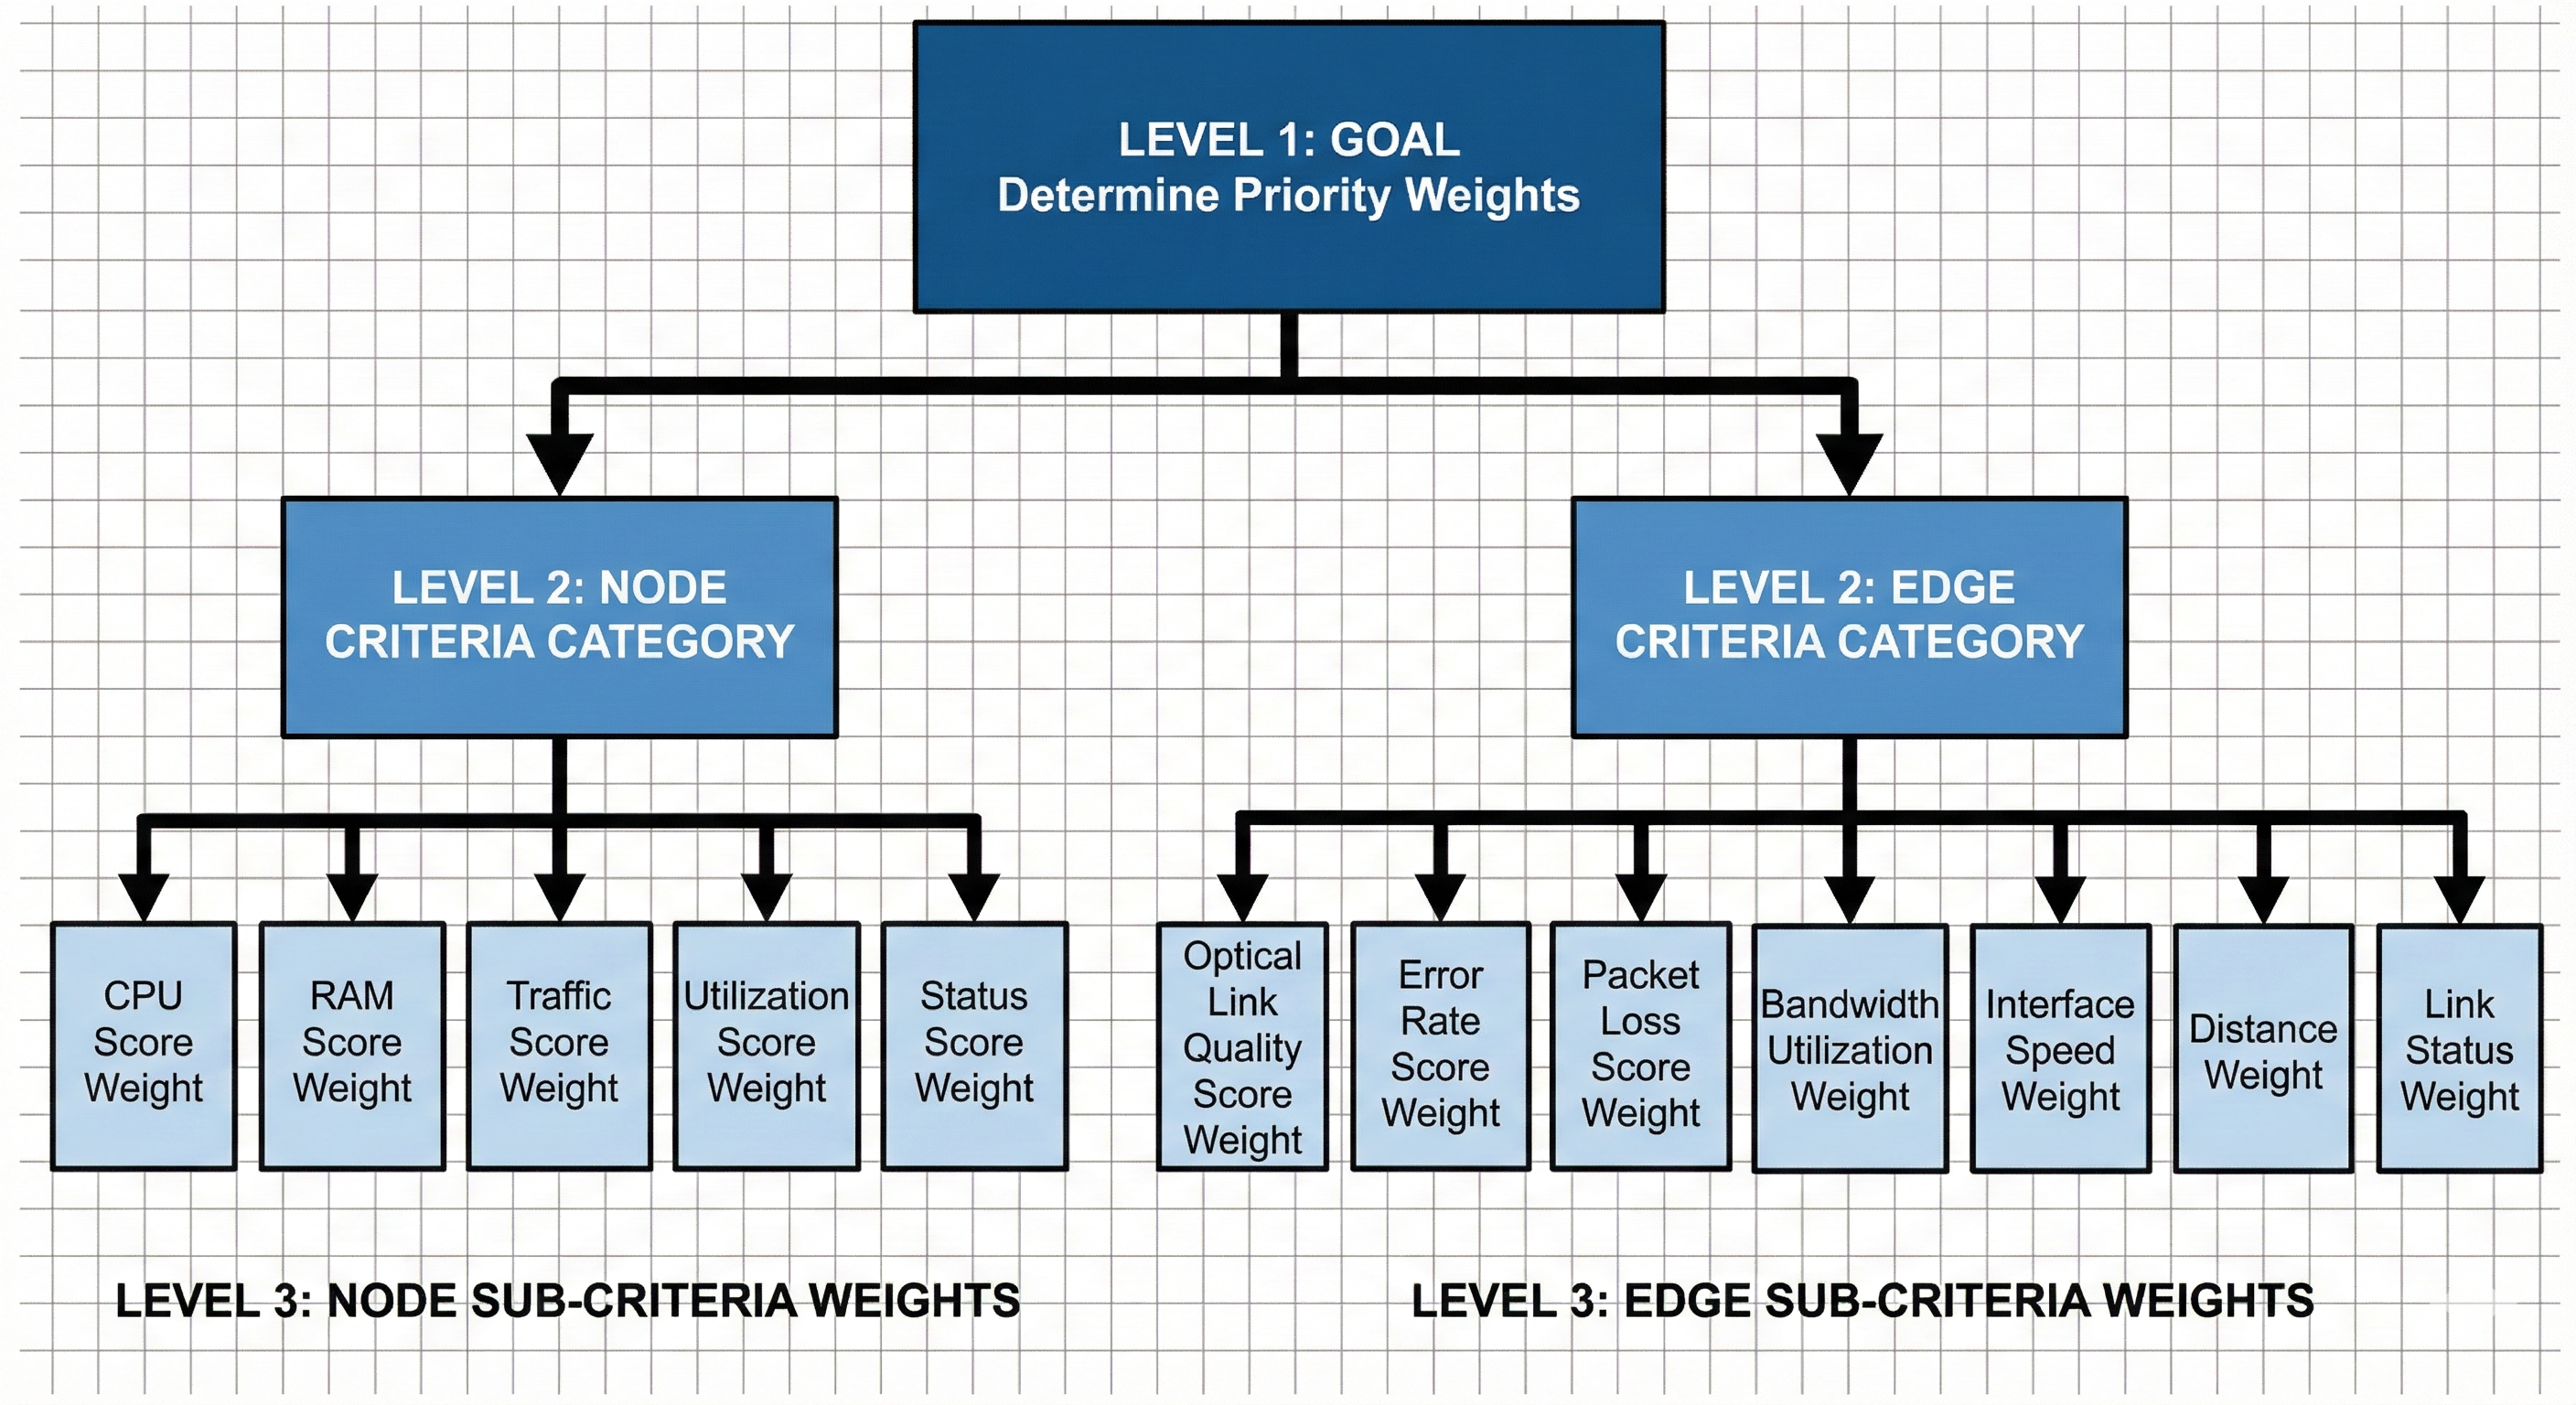
\includegraphics[width=0.9\textwidth]{images/hirarki.png}
    \caption{Struktur Hierarki AHP untuk Penentuan Bobot Parameter}
    \label{fig:ahp_hierarchy}
\end{figure}

\subsubsection{Tahapan Metode AHP}
Implementasi AHP meliputi lima tahapan sistematis yang dijelaskan berikut ini:

\paragraph{1. Penyusunan Matriks Perbandingan Berpasangan}
Matriks perbandingan disusun dengan membandingkan setiap pasangan kriteria berdasarkan skala Saaty. Matriks berukuran $n \times n$ ini bersifat resiprokal:

\begin{equation}
    \mathbf{A} = \begin{bmatrix}
        1 & a_{12} & \cdots & a_{1n} \\
        1/a_{12} & 1 & \cdots & a_{2n} \\
        \vdots & \vdots & \ddots & \vdots \\
        1/a_{1n} & 1/a_{2n} & \cdots & 1
    \end{bmatrix}, \quad a_{ji} = \frac{1}{a_{ij}}
\end{equation}
\noindent dengan:
\begin{itemize}[label={}, leftmargin=1.5cm, labelsep=0.5cm, noitemsep]
    \item[$\mathbf{A}$] : Matriks perbandingan berpasangan AHP
    \item[$a_{ij}$] : Nilai perbandingan kepentingan kriteria $i$ terhadap kriteria $j$
    \item[$n$] : Jumlah kriteria yang dibandingkan
\end{itemize}

Skala penilaian mengikuti standar Saaty seperti ditunjukkan Tabel \ref{tab:saaty_scale}.

\begin{table}[H]
\centering
\caption{Skala Perbandingan Berpasangan Saaty}
\label{tab:saaty_scale}
\begin{tabular}{|c|l|}
\hline
\textbf{Nilai} & \textbf{Interpretasi} \\
\hline
1 & Kedua elemen sama pentingnya \\
3 & Elemen pertama sedikit lebih penting \\
5 & Elemen pertama lebih penting \\
7 & Elemen pertama sangat lebih penting \\
9 & Elemen pertama mutlak lebih penting \\
2, 4, 6, 8 & Nilai antara untuk kompromi \\
\hline
\end{tabular}
\end{table}

\paragraph{2. Normalisasi Matriks Perbandingan}
Setiap kolom matriks dinormalisasi dengan membagi setiap elemen terhadap total kolomnya:

\begin{equation}
    T_j = \sum_{i=1}^{n} a_{ij}, \quad n_{ij} = \frac{a_{ij}}{T_j}
\end{equation}
\noindent dengan:
\begin{itemize}[label={}, leftmargin=1.5cm, labelsep=0.5cm, noitemsep]
    \item[$T_j$] : Total jumlah nilai pada kolom $j$
    \item[$n_{ij}$] : Nilai elemen matriks yang telah dinormalisasi
\end{itemize}

\paragraph{3. Perhitungan Vektor Prioritas dan Bobot}
Vektor prioritas diperoleh dari rata-rata baris matriks ternormalisasi:

\begin{equation}
    PV_i = \sum_{j=1}^{n} n_{ij}, \quad w_i = \frac{PV_i}{n}
\end{equation}
\noindent dengan:
\begin{itemize}[label={}, leftmargin=1.5cm, labelsep=0.5cm, noitemsep]
    \item[$PV_i$] : Nilai prioritas (jumlah baris ternormalisasi)
    \item[$w_i$] : Bobot prioritas akhir untuk kriteria $i$
\end{itemize}

\paragraph{4. Uji Konsistensi}

Langkah pertama dalam uji konsistensi adalah menghitung nilai eigen maksimum ($\lambda_{max}$) yang diperoleh dari rata-rata rasio antara vektor konsistensi ($CV$) dengan bobot prioritas ($w$):

\begin{equation}
    \lambda_{max} = \frac{1}{n} \sum_{i=1}^{n} \frac{CV_i}{w_i}
\end{equation}
\noindent dengan:
\begin{itemize}[label={}, leftmargin=1.5cm, labelsep=0.5cm, noitemsep]
    \item[$\lambda_{max}$] : Nilai eigen maksimum dari matriks perbandingan
    \item[$CV_i$] : Elemen vektor konsistensi baris ke-$i$ (hasil perkalian matriks dengan bobot)
    \item[$w_i$] : Bobot prioritas kriteria ke-$i$
    \item[$n$] : Jumlah kriteria (orde matriks)
\end{itemize}

Selanjutnya, dihitung nilai \textit{Consistency Index} (CI) untuk mengukur penyimpangan konsistensi data:

\begin{equation}
    CI = \frac{\lambda_{max} - n}{n - 1}
\end{equation}
\noindent dengan:
\begin{itemize}[label={}, leftmargin=1.5cm, labelsep=0.5cm, noitemsep]
    \item[$CI$] : \textit{Consistency Index}
    \item[$\lambda_{max}$] : Nilai eigen maksimum
    \item[$n$] : Jumlah elemen atau kriteria yang dibandingkan
\end{itemize}

Terakhir, rasio konsistensi atau \textit{Consistency Ratio} (CR) dihitung dengan membandingkan nilai CI terhadap \textit{Random Index} (RI):

\begin{equation}
    CR = \frac{CI}{RI}
\end{equation}
\noindent dengan:
\begin{itemize}[label={}, leftmargin=1.5cm, labelsep=0.5cm, noitemsep]
    \item[$CR$] : \textit{Consistency Ratio}
    \item[$RI$] : \textit{Random Consistency Index}
\end{itemize}

Nilai referensi untuk \textit{Random Index} (RI) bergantung pada jumlah kriteria ($n$) yang digunakan, seperti yang disajikan pada Tabel \ref{tab:ri_index}.

\begin{table}[H]
\centering
\caption{Nilai Random Index (RI)}
\label{tab:ri_index}
\begin{tabular}{|c|c|c|c|c|c|c|c|c|c|c|}
\hline
\textbf{n} & 1 & 2 & 3 & 4 & 5 & 6 & 7 & 8 & 9 & 10 \\
\hline
\textbf{RI} & 0 & 0 & 0{,}58 & 0{,}90 & 1{,}12 & 1{,}24 & 1{,}32 & 1{,}41 & 1{,}45 & 1{,}49 \\
\hline
\end{tabular}
\end{table}

Suatu matriks perbandingan dinyatakan konsisten dan dapat diterima jika nilai $CR \leq 0{,}1$. Jika nilai $CR > 0{,}1$, maka penilaian perbandingan berpasangan perlu diperbaiki ulang.

\paragraph{5. Output Bobot AHP}
Tahap ini menghasilkan vektor bobot final $\mathbf{w}_{node}$ dan $\mathbf{w}_{edge}$ yang siap diintegrasikan ke dalam perhitungan skor kualitas jalur.

\subsection{Graph Attention Network (GAT)}

\textit{Graph Attention Network} (GAT) merupakan evolusi dari \textit{Graph Neural Networks} (GNN) yang mengintegrasikan mekanisme \textit{masked self-attention} untuk mengatasi keterbatasan pendekatan berbasis graf konvensional \cite{velickovic2017}. GAT memungkinkan model untuk "memfokuskan perhatian" pada jalur dengan kualitas superior dan mengurangi pengaruh jalur yang mengalami degradasi \cite{kato2024}.

\subsubsection{Representasi Graf Jaringan}

Topologi jaringan dimodelkan sebagai graf tidak berarah $\mathcal{G} = (\mathcal{V}, \mathcal{E})$. Setiap node $v_i \in \mathcal{V}$ memiliki vektor fitur $\vec{h}_i$, sementara setiap edge $e_{ij} \in \mathcal{E}$ memiliki atribut $\vec{f}_{ij}$.

\paragraph{Struktur Konektivitas Graf}
Konektivitas antar node direpresentasikan melalui matriks adjacency $\mathbf{A}$. Himpunan tetangga node $i$ didefinisikan sebagai:

\begin{equation}
    \mathcal{N}_i = \{v_j \in \mathcal{V} : A_{ij} = 1\}
\end{equation}
\noindent dengan:
\begin{itemize}[label={}, leftmargin=1.5cm, labelsep=0.5cm, noitemsep]
    \item[$\mathcal{N}_i$] : Himpunan node tetangga yang terhubung langsung ke node $i$
    \item[$A_{ij}$] : Elemen matriks adjacency ($1$ jika terhubung, $0$ jika tidak)
\end{itemize}

\paragraph{Integrasi Fitur Edge dalam GAT}
Penelitian ini mengadopsi strategi \textbf{Edge Feature Concatenation}, dimana fitur edge digabungkan dengan fitur node dalam perhitungan skor attention:

\begin{equation}
    s_{ij} = \text{LeakyReLU}\left(\vec{a}^T [\mathbf{W}\vec{h}_i \, \| \, \mathbf{W}\vec{h}_j \, \| \, \mathbf{W}_e\vec{f}_{ij}]\right)
\end{equation}
\noindent dengan:
\begin{itemize}[label={}, leftmargin=1.5cm, labelsep=0.5cm, noitemsep]
    \item[$s_{ij}$] : Skor attention awal yang melibatkan fitur edge
    \item[$\vec{a}$] : Vektor parameter weight vector untuk mekanisme attention
    \item[$\mathbf{W}, \mathbf{W}_e$] : Matriks transformasi linear untuk fitur node dan edge
    \item[$\vec{h}, \vec{f}$] : Vektor fitur node dan vektor fitur edge
    \item[$\|$] : Operasi concatenation (penggabungan)
\end{itemize}

\subsubsection{Tahapan Komputasi GAT}

\paragraph{1. Transformasi Linear Fitur Input}
Fitur input setiap node ditransformasi ke ruang fitur yang lebih ekspresif:
\begin{equation}
    \vec{z}_i = \mathbf{W} \vec{h}_i
\end{equation}
\noindent dengan:
\begin{itemize}[label={}, leftmargin=1.5cm, labelsep=0.5cm, noitemsep]
    \item[$\vec{z}_i$] : Fitur node $i$ setelah transformasi linear
    \item[$\mathbf{W}$] : Matriks bobot yang dipelajari (learnable weight matrix)
\end{itemize}

\paragraph{2. Komputasi Skor Attention Mentah}
Kepentingan relatif node tetangga $j$ terhadap node $i$ dihitung menggunakan mekanisme attention:
\begin{equation}
    e_{ij} = \text{LeakyReLU}\left(\vec{a}^T [\vec{z}_i \, \| \, \vec{z}_j]\right)
\end{equation}
\noindent dengan:
\begin{itemize}[label={}, leftmargin=1.5cm, labelsep=0.5cm, noitemsep]
    \item[$e_{ij}$] : Koefisien attention mentah (belum dinormalisasi)
\end{itemize}

Fungsi LeakyReLU didefinisikan sebagai:
\begin{equation}
    \text{LeakyReLU}(x) = \begin{cases}
        x & \text{jika } x \geq 0 \\
        \lambda x & \text{jika } x < 0
    \end{cases}
\end{equation}
\noindent dengan:
\begin{itemize}[label={}, leftmargin=1.5cm, labelsep=0.5cm, noitemsep]
    \item[$\lambda$] : Slope untuk nilai negatif (biasanya 0.01 - 0.2)
\end{itemize}

\paragraph{3. Normalisasi dengan Softmax}
Skor attention mentah dinormalisasi menjadi distribusi probabilitas:
\begin{equation}
    \alpha_{ij} = \text{softmax}_j(e_{ij}) = \frac{\exp(e_{ij})}{\sum_{k \in \mathcal{N}_i \cup \{i\}} \exp(e_{ik})}
\end{equation}
\noindent dengan:
\begin{itemize}[label={}, leftmargin=1.5cm, labelsep=0.5cm, noitemsep]
    \item[$\alpha_{ij}$] : Koefisien attention ternormalisasi (tingkat kepentingan node $j$ bagi $i$)
\end{itemize}

\paragraph{4. Agregasi Fitur dengan Weighted Sum}
Informasi dari node tetangga diagregasi menggunakan weighted sum:
\begin{equation}
    \vec{h'}_i = \sigma\left(\sum_{j \in \mathcal{N}_i \cup \{i\}} \alpha_{ij} \vec{z}_j\right)
\end{equation}
\noindent dengan:
\begin{itemize}[label={}, leftmargin=1.5cm, labelsep=0.5cm, noitemsep]
    \item[$\vec{h'}_i$] : Fitur output node $i$
    \item[$\sigma$] : Fungsi aktivasi non-linear (misalnya ELU)
\end{itemize}

\paragraph{5. Multi-Head Attention}
Output dari $K$ heads digabungkan melalui concatenation:
\begin{equation}
    \vec{h'}_i = \Bigg\|_{k=1}^{K} \sigma\left(\sum_{j \in \mathcal{N}_i \cup \{i\}} \alpha_{ij}^k \mathbf{W}^k\vec{h}_j\right)
\end{equation}

Untuk output layer (prediksi final), digunakan averaging:
\begin{equation}
    \vec{h'}_i = \sigma\left(\frac{1}{K}\sum_{k=1}^{K} \sum_{j \in \mathcal{N}_i \cup \{i\}} \alpha_{ij}^k \mathbf{W}^k\vec{h}_j\right)
\end{equation}
\noindent dengan:
\begin{itemize}[label={}, leftmargin=1.5cm, labelsep=0.5cm, noitemsep]
    \item[$K$] : Jumlah attention heads yang berjalan paralel
    \item[$\alpha_{ij}^k$] : Koefisien attention pada head ke-$k$
\end{itemize}

\subsection{Integrasi AHP dengan GAT}

Penelitian ini mengintegrasikan AHP dengan GAT melalui mekanisme \textit{Expert-Guided Feature Weighting}.

\subsubsection{Perhitungan Skor Kualitas Node dan Edge}
Skor kualitas setiap komponen jaringan dihitung menggunakan weighted sum:

\begin{equation}
    Q_{node}(v) = \sum_{k=1}^{6} w_k^{node} \cdot s_k(v)
\end{equation}

\begin{equation}
    Q_{edge}(e) = \sum_{k=1}^{7} w_k^{edge} \cdot s_k(e)
\end{equation}
\noindent dengan:
\begin{itemize}[label={}, leftmargin=1.5cm, labelsep=0.5cm, noitemsep]
    \item[$Q_{node}(v)$] : Skor kualitas node $v$
    \item[$Q_{edge}(e)$] : Skor kualitas edge $e$
    \item[$s_k$] : Nilai parameter ke-$k$ yang telah dinormalisasi
\end{itemize}

\subsubsection{Perhitungan Skor Kualitas Jalur}
Skor kualitas jalur secara keseluruhan dihitung dengan pendekatan weighted average yang dimodifikasi dengan penalti hop:

\begin{equation}
    Q_{path} = \left( \frac{\sum_{v \in P} Q_{node}(v) + \sum_{e \in P} Q_{edge}(e)}{|P|_{components}} \right) \times (1 - \text{Penalty}_{hop})
\end{equation}
\noindent dengan:
\begin{itemize}[label={}, leftmargin=1.5cm, labelsep=0.5cm, noitemsep]
    \item[$Q_{path}$] : Skor kualitas jalur keseluruhan
    \item[$P$] : Himpunan node dan edge dalam jalur
    \item[$|P|_{components}$] : Jumlah total komponen (node + edge) dalam jalur
\end{itemize}

Penalti hop didefinisikan sebagai:
\begin{equation}
    \text{Penalty}_{hop} = \alpha \cdot \frac{h}{h_{max}}
\end{equation}
\noindent dengan:
\begin{itemize}[label={}, leftmargin=1.5cm, labelsep=0.5cm, noitemsep]
    \item[$\alpha$] : Koefisien sensitivitas penalti
    \item[$h$] : Jumlah hop pada jalur saat ini
    \item[$h_{max}$] : Jumlah hop maksimum dalam topologi jaringan
\end{itemize}

\subsubsection{Alur Kerja Integrasi AHP-GAT}
Gambar \ref{fig:ahp_gat_integration} mengilustrasikan alur kerja lengkap integrasi AHP dengan GAT.

\begin{figure}[H]
    \centering
    \resizebox{0.95\textwidth}{!}{%
    \begin{tikzpicture}[
        node distance=1.2cm and 1.5cm,
        box/.style={
            rectangle,
            rounded corners,
            draw=black!70,
            minimum width=3.5cm,
            minimum height=1cm,
            align=center,
            font=\small,
            fill=white,
            drop shadow
        },
        databox/.style={
            box,
            fill=blue!10
        },
        processbox/.style={
            box,
            fill=green!10
        },
        resultbox/.style={
            box,
            fill=orange!10
        },
        arrow/.style={
            ->,
            thick,
            >=stealth,
            color=black!70
        },
        labelstyle/.style={
            font=\bfseries\small,
            align=center
        }
    ]

    % ===== STAGE 1: EXPERT WEIGHTING =====
    \node[processbox] (expert) {Expert\\Judgment};
    \node[processbox, below=of expert] (ahp) {\textbf{AHP Process}\\Pairwise Comparison\\Consistency Check};
    \node[databox, below=of ahp] (weights) {Weight Vectors\\$\mathbf{w}_{node} \in \mathbb{R}^6$\\$\mathbf{w}_{edge} \in \mathbb{R}^7$};

    % ===== STAGE 2: RULE-BASED LABELING =====
    \node[databox, right=2cm of expert] (features) {Network Metrics\\Node Features\\Edge Features};
    \node[processbox, below=of features] (scoring) {\textbf{Rule-Based Scoring}\\Weighted Sum\\Hop Penalty};
    \node[databox, below=of scoring] (labels) {Ground Truth\\$Q_{path}$ Labels\\(Target Values)};

    % ===== STAGE 3: GAT TRAINING =====
    \node[processbox, right=2cm of features] (gat) {\textbf{GAT Training}\\Multi-Head Attention\\Graph Convolution\\MSE Loss};
    \node[resultbox, below=of gat] (model) {Trained Model\\Path Quality\\Predictor};

    % ===== STAGE 4: INFERENCE =====
    \node[databox, right=1.5cm of gat] (newdata) {New Network\\State\\(Real-time)};
    \node[resultbox, below=of newdata] (prediction) {Path Quality\\Prediction\\$\hat{Q}_{path}$};

    % ===== ARROWS STAGE 1 =====
    \draw[arrow] (expert) -- (ahp) node[midway, right, font=\scriptsize] {preferences};
    \draw[arrow] (ahp) -- (weights) node[midway, right, font=\scriptsize] {validated};

    % ===== ARROWS STAGE 2 =====
    \draw[arrow] (weights) -- (scoring) node[midway, above, font=\scriptsize] {apply};
    \draw[arrow] (features) -- (scoring) node[midway, right, font=\scriptsize] {input};
    \draw[arrow] (scoring) -- (labels) node[midway, right, font=\scriptsize] {compute};

    % ===== ARROWS STAGE 3 =====
    \draw[arrow] (features) -- (gat) node[midway, above, font=\scriptsize] {features};
    \draw[arrow] (labels) -- (gat) node[midway, above, font=\scriptsize] {targets};
    \draw[arrow] (gat) -- (model) node[midway, right, font=\scriptsize] {optimize};

    % ===== ARROWS STAGE 4 =====
    \draw[arrow] (model) -- (prediction) node[midway, above, font=\scriptsize] {inference};
    \draw[arrow] (newdata) -- (prediction) node[midway, right, font=\scriptsize] {input};

    % ===== STAGE LABELS =====
    \node[labelstyle, above=0.4cm of expert] {Stage 1\\Expert Weighting};
    \node[labelstyle, above=0.4cm of features] {Stage 2\\Rule-Based Labeling};
    \node[labelstyle, above=0.4cm of gat] {Stage 3\\Supervised Learning};
    \node[labelstyle, above=0.4cm of newdata] {Stage 4\\Real-time Inference};

    % ===== DASHED GROUPING BOXES =====
    \node[draw=blue!50, dashed, rounded corners, fit=(expert)(ahp)(weights),
          inner sep=0.3cm, label={[anchor=south, font=\scriptsize]below:AHP Module}] {};
    \node[draw=green!50, dashed, rounded corners, fit=(features)(scoring)(labels),
          inner sep=0.3cm, label={[anchor=south, font=\scriptsize]below:Labeling Module}] {};
    \node[draw=orange!50, dashed, rounded corners, fit=(gat)(model),
          inner sep=0.3cm, label={[anchor=south, font=\scriptsize]below:Learning Module}] {};
    \node[draw=red!50, dashed, rounded corners, fit=(newdata)(prediction),
          inner sep=0.3cm, label={[anchor=south, font=\scriptsize]below:Deployment Module}] {};

    \end{tikzpicture}%
    }
    \caption{Alur Integrasi AHP dengan GAT dalam Sistem Rekomendasi Jalur}
    \label{fig:ahp_gat_integration}
\end{figure}

Penjelasan detail setiap tahapan adalah sebagai berikut:

\begin{enumerate}
    \item \textbf{Stage 1 - Expert Weighting}: Pakar jaringan melakukan penilaian AHP untuk menghasilkan vektor bobot $\mathbf{w}_{node}$ dan $\mathbf{w}_{edge}$.
    \item \textbf{Stage 2 - Rule-Based Labeling}: Sistem menghitung skor $Q_{path}$ sebagai ground truth sintetis.
    \item \textbf{Stage 3 - Supervised Learning}: Model GAT dilatih untuk meminimalkan loss Mean Squared Error (MSE):
        \begin{equation}
            \mathcal{L} = \frac{1}{N} \sum_{i=1}^{N} \left(Q_{pred}^{(i)} - Q_{target}^{(i)}\right)^2
        \end{equation}
        \noindent dengan:
        \begin{itemize}[label={}, leftmargin=1.5cm, labelsep=0.5cm, noitemsep]
            \item[$\mathcal{L}$] : Nilai Loss Function (MSE)
            \item[$N$] : Jumlah sampel data training
            \item[$Q_{pred}$] : Prediksi kualitas jalur dari model GAT
            \item[$Q_{target}$] : Label kualitas jalur (Ground Truth) dari Stage 2
        \end{itemize}
    \item \textbf{Stage 4 - Real-time Inference}: Model memprediksi kualitas jalur $\hat{Q}_{path}$ secara real-time.
\end{enumerate}

\section{Penelitian Terkait}
% (Bagian ini tetap sama seperti sebelumnya, tidak ada perubahan rumus)
Tinjauan studi dilakukan untuk memetakan posisi penelitian ini terhadap penelitian-penelitian sebelumnya yang relevan... (Lanjutan teks asli Anda)

\begin{table}[ht]
    \centering
    \caption{State of the Art Penelitian}
    \label{tab:state_of_the_art}
    \small
    \begin{tabular}{p{3cm} p{3cm} p{2.5cm} p{4.5cm}}
        \hline
        \textbf{Peneliti (Tahun)} & \textbf{Masalah} & \textbf{Metode} & \textbf{Hasil \& Perbedaan} \\
        \hline
        \cite{marouani2024} & Optimasi trafik pada WAN & GAT & Unggul di topologi dinamis. \textbf{Bedanya:} Penelitian ini menambahkan validasi pakar via AHP. \\
        \hline
       \cite{almasan2022} & Optimasi \textit{Routing} & DRL + GNN & Generalisasi baik tapi training berat. \textbf{Bedanya:} Penelitian ini menggunakan \textit{Supervised Learning} yang lebih efisien. \\
        \hline
        \cite{rahman2023} & Prediksi Trafik & GCN & Efektif spasial. \textbf{Bedanya:} GAT memiliki mekanisme \textit{attention} yang lebih presisi dibanding GCN. \\
        \hline
        \textbf{Penelitian Ini} & \textbf{Rekomendasi Jalur ISP} & \textbf{GAT + AHP} & \textbf{Integrasi \textit{expert judgment} (AHP) ke dalam arsitektur \textit{Deep Learning} (GAT).} \\
        \hline
    \end{tabular}
\end{table}

\section{Kerangka Pemikiran}
% (Bagian ini tetap sama seperti sebelumnya)
Kerangka pemikiran menggambarkan alur logika penelitian dari variabel yang diobservasi hingga pengukuran keberhasilan... (Lanjutan teks asli Anda)

\begin{figure}[ht]
    \centering
    \resizebox{\textwidth}{!}{%
    \begin{tikzpicture}[
        node distance=0.6cm and 0.8cm, % Jarak Vertikal dan Horizontal
        box/.style={
            rectangle,
            draw=black!70,
            rounded corners,
            minimum width=3.5cm,
            minimum height=1cm,
            align=center,
            font=\small,
            fill=white,
            drop shadow
        },
        header/.style={
            font=\bfseries\large,
            align=center
        },
        groupbox/.style={
            draw=black!50,
            rounded corners,
            dashed,
            inner sep=0.4cm,
            align=center
        },
        arrow/.style={
            ->,
            thick,
            >=stealth,
            color=black!80
        }
    ]

    % --- COLUMN 1: INDICATORS ---
    \node[header] (ind_title) {INDICATORS};
    \node[box, below=0.5cm of ind_title] (cpu) {CPU \& RAM\\Usage};
    \node[box, below=of cpu] (traf) {Traffic \&\\Utilization};
    \node[box, below=of traf] (link) {Optical Quality\\Error Rate};
    \node[box, below=of link] (bw) {Bandwidth\\Availability};
    \node[box, below=of bw] (dist) {Distance \&\\Status};
    \node[groupbox, fit=(cpu)(dist), label={[anchor=north]below:\textit{Observed Variables}}] (ind_group) {};

    % --- COLUMN 2: PROPOSED METHOD ---
    \node[header, right=2cm of ind_title] (met_title) {PROPOSED METHOD};
    \node[box, below=0.5cm of met_title, fill=gray!10] (data) {Dataset Generation\\(Topology \& Metrics)};
    \node[box, below=of data, fill=gray!10] (ahp) {\textbf{Weighting Strategy}\\Analytic Hierarchy Process\\(AHP)};
    \node[box, below=of ahp, dashed, fill=yellow!10] (labeling) {\textbf{Label Generation}\\Rule-Based Scoring\\(Weighted Sum + Penalty)};
    \node[box, below=of labeling, fill=blue!10, minimum height=1.5cm] (gat) {\textbf{Learning Algorithm}\\Graph Attention Network\\(Multi-Head Attention)};
    \node[box, below=of gat, fill=gray!10] (pred) {Path Quality\\Predictor};
    \node[groupbox, fit=(data)(pred)] (met_group) {};

    % --- COLUMN 3: OBJECTIVES ---
    \node[header, right=1.5cm of met_title] (obj_title) {OBJECTIVES};
    \node[circle, draw, align=center, minimum size=2.8cm, fill=white, drop shadow, right=1.5cm of labeling, yshift=1cm] (obj1) {High Accuracy\\Model};
    \node[circle, draw, align=center, minimum size=2.8cm, fill=white, drop shadow, below=0.5cm of obj1] (obj2) {Optimal Path\\Recommendation};

    % --- COLUMN 4: MEASUREMENT ---
    \node[header, right=1.5cm of obj_title] (meas_title) {MEASUREMENT};
    \node[box, below=1.5cm of meas_title] (rmse) {Root Mean\\Square Error (RMSE)};
    \node[box, below=of rmse] (acc) {Model\\Accuracy};
    \node[box, below=of acc] (time) {Inference Time};
    \node[groupbox, fit=(rmse)(time), label={[anchor=north]below:\textit{Observed Results}}] (meas_group) {};

    % --- ARROWS (ALUR) ---
    \draw[arrow, dashed] (ind_group.east) -- (met_group.west);
    \draw[arrow] (data) -- (ahp);
    \draw[arrow] (ahp) -- (labeling);
    \draw[arrow] (labeling) -- (gat);
    \draw[arrow] (gat) -- (pred);
    \draw[arrow] (met_group.east) -- (obj1.west);
    \draw[arrow] (met_group.east) -- (obj2.west);
    \draw[arrow] (obj1.east) -- (rmse.west);
    \draw[arrow] (obj1.east) -- (acc.west);
    \draw[arrow] (obj2.east) -- (time.west);

    \end{tikzpicture}%
    }
    \caption{Kerangka Pemikiran Sistem Rekomendasi Jalur (GAT-AHP)}
    \label{fig:kerangka_pemikiran}
\end{figure}
